% Created:  Mon 01 Sep 2014 01:03 PM
% Author:   Josh Wainwright
% Filename: testing.tex

\section{Testing}
\label{sec:testing}

Since the absolute definition of the clusters that the plugin looks for are
somewhat subjective, testing the algorithm for correctness is difficult. The
individual functions and smaller components of the algorithms are tested using
the unit testing framework JUnit\cite{tahchiev2010junit}, and the overall
effectiveness of the clustering algorithms is validated with generated data
files and acceptance testing.

\subsection{Generated Test Files}
\label{sub:generated_test_files}

To try to test the algorithm and get some more quantitative results, it was
performed on a number of simulated test files. These data sets, shown in
Figure~\ref{fig:cam-tests} were produced by \citet{karypis1999chameleon} for
testing their Cameleon clustering algorithm. The algorithm was found to
identify 4 clusters in image (a) and a single cluster image (b), but performed
poorly in the final two.

\begin{figure}[tbh]
	\centering
	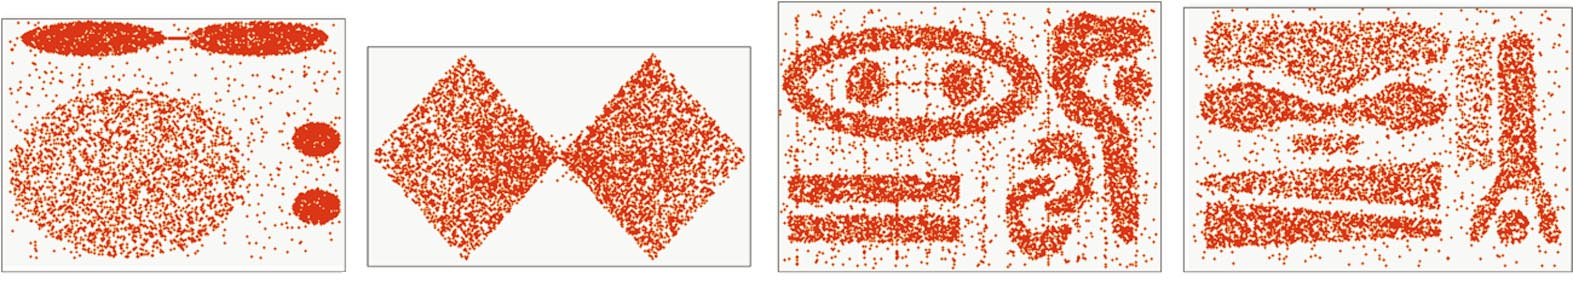
\includegraphics[width=0.9\linewidth]{cam-tests.png}
	\caption[Manually generated data sets for testing]{Manually generated data
		sets for testing. The images (a), (b), (c) and (d) above are used to
		test the algorithm for this project and for a number of other studies
		in clustering.}\label{fig:cam-tests}
\end{figure}

These particular datasets have been used to test a number of clustering
algorithms and so they provide a helpful benchmark with which these algorithms
can be compared. It is unfortunate that this algorithm fails to cope with the
complex structures that are present in the second two images, but shows that it
is more specifically taylored than the more general algorithms that use these
as tests. The clusters that the algorithm failed to identify lie too close
together meaning that the propagation step is able to cross from one cluster to
another.

The same effect is seen in images (a) and (b) where there is a link between
what would, otherwise, be separate clusters. This means the algorithm reports
these as a single object.

Another testing data set was created, similar to the final two images above,
but with more spacing to see how the algorithm would cope. An image of this set
is shown in Figure~\ref{fig:testing-image2a}.

\begin{figure}[tbh]
	\centering
	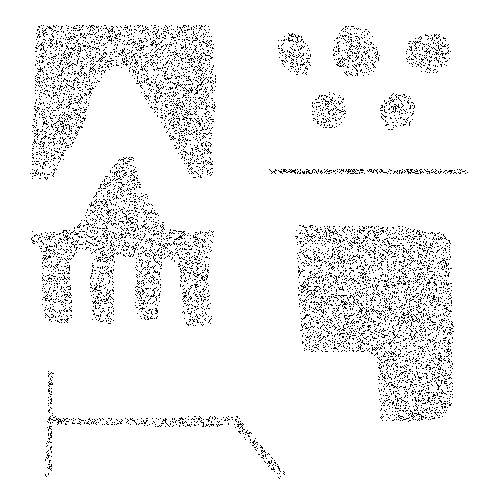
\includegraphics[width=0.5\linewidth]{testing-image2a.png}
	\caption[Custom generated data set for testing clustering
		algorithm.]{Custom generated data set for testing clustering
		algorithm. This data set is similar to that shown above, but
		has more space between clusters. The number of points in this
		% TODO Number of points in dataset.
		data set is .} \label{fig:testing-image2a}
\end{figure}

The results were better with this data set since the propagation step of the
algorithm was halted by the clear space between the clusters. When there is no
noise at all in the data, all of the clusters are located. The amount of noise
can be increased by simply adding random data points which are distributed
evenly across the image space. This is done progressively, adding TODO points
at a time. The clustering algorithm stops finding the clusters properly when
the number of noise points added is TODO. This represents when the noise to
signal ratio is TODO.

\subsection{Volunteer Validation}
\label{sub:volunteer_validation}

The first stage of acceptance testing took the form of a sample set of data
that was plotted onto an image using the discrete grid method. This data was
then presented to a number of volunteers who were asked to count the number of
clusters they could identify and then highlight the clusters that they were
able to observe in order of precedence, most defined through to least defined.

Once the volunteer had identified the clusters, the algorithm was performed on
the same set of data and the results compared to the predicted results.
Finally, when the algorithm identified clusters that the volunteers had not,
they were asked to identify which of these they did not consider to be valid
clusters and which were valid clusters that they had missed. The number of
false positive clusters identified by the quadtree algorithm was found, by this
method, to be low.

When using the settings described in Section~\ref{sub:option_sliders}, 100\% of
the clusters identified by the volunteers were able to be located by the
algorithm. Of the clusters that the algorithm found but the volunteers did not,
around 60\% were considered to be valid by the volunteers. These results
suggest that the algorithm is performing well at being able to identify
clusters, but requires some intervention to get the best results (see
Section~\ref{sec:possible_improvements}) and that, in general, the algorithm
does not produce that many false positive results.

\subsection{Researcher Validation}
\label{sub:researcher_validation}

The final stage of acceptance testing was performed to confirm the type of
clusters identified conformed with the actual objects that are being imaged.
This was performed by two researchers working in the medical imaging field who
produced the sample data used in this project.
% TODO
